\chapter{肾上腺}

\section{检查方法}

\subsection{扫描前准备}

与腹部其他器官的CT检查方法相似。扫描前10~20分钟口服1%~2%的泛影葡胺500~800ml,临扫描前再口服200ml,以充盈胃、十二指肠及小肠。增强扫描者同其他常规准备。

\subsection{扫描方法}

①患者仰卧位,通常扫描上界定在T\textsubscript{11}
下缘,下缘定在L\textsubscript{1~2}
之间,应包括双肾上极,最好至肾门。②扫描层厚和层间距一般为3~5mm。对怀疑醛固酮增多症者,扫描层厚和层间距可为1.5~3mm,甚至重叠扫描,以防1cm以下的肿物漏诊。当发现较大肿物时,层厚和层间距可用8~10mm。③当怀疑异位嗜铬细胞瘤时,应加扫胸、腹或盆腔。④一般不需做增强扫描,但为了鉴别良恶性,可行增强扫描。增强扫描还有利于条状血管影与肾上腺肢体的区分。⑤当有嗜铬细胞瘤时增强扫描注射速度应减缓,以免发生高血压危象。⑥为了鉴别肿物是否来自肾上腺,可作矢状、冠状面成像。

此外,螺旋CT扫描一般采用螺距1~1.5,层厚5~10mm,必要时扫描后再作2~3mm薄层重建。

\section{正常解剖和CT表现}

\subsection{大小和变异}

1.位置与形态:左右肾上腺位于腹膜后,居双侧肾上极之前上方,包在肾筋膜内,周围有丰富的脂肪。肾上腺相当于L\textsubscript{1}
水平,右侧较左侧略高。①右侧肾上腺:呈锥形或三角形。位于下腔静脉后,外侧是肝、内侧是膈肌脚。②左侧肾上腺:通常呈椭圆形或半月形。位于胰体尾和脾静脉之后、左膈肌脚之外侧,其顶端常位于左肾上极之前内侧。

2.大小:肾上腺长(上下径)4~6cm,宽2~4cm,厚0.3~0.6cm。由外面的皮质和中间的髓质组成,皮质和髓质之比为(8~9)∶1。

3.变异:副上腺或附属肾上腺,又称异位肾上腺组织,为正常变异,见于少数人。分布范围很广,主要位于肾脏和肾上腺周围。

\subsection{肾上腺的组织学结构和功能}

肾上腺由皮质和髓质组成,两者起源不同,前者起源于中胚层,后者起源于外胚层;而且两者组织形态、功能也不相同,可视为两个独立的内分泌腺。

肾上腺皮质按细胞形态和排列方式由外向内分为球状带、束状带和网状带3层。球状带产生调节电解质和水盐代谢的皮质激素,以醛固酮为代表。束状带分泌调节糖和蛋白质代谢的皮质激素,以皮质醇为代表。网状带分泌性激素,主要为雄激素,也有少量雌激素。束状带和网状带在功能上均受垂体分泌的促肾上腺皮质激素(ACTH)的调节。

肾上腺髓质几乎完全由嗜铬细胞组成,分泌肾上腺素和去甲肾上腺素,统称为儿茶酚胺。

\subsection{肾上腺的CT表现和测量}

1.正常CT表现:肾上腺可分成内侧肢、外侧肢以及由内外侧肢相交构成的体部。根据横断扫描层面以及肾上腺与扫描层面所成角度,其CT形态多样,基本可分为:三角形、倒V字形或“人”字形及线形,少数呈Y形,逗点形或蝌蚪形。右侧以线条形最多见,三角形很少见;左侧以倒V字形或人字形最多见,其次是三角形。

右肾上腺通常位于右肾上方1~2cm高度,并向下延伸3~4cm,位于下腔静脉后方、右膈肌脚与肝右叶内缘之间。右肾上腺外侧缘常与肝右叶内缘重叠而难以显示。左肾上腺位于主动脉左侧、胰腺和脾静脉的后方,其头端常位于左肾上极的前内侧。

2.大小测量:肢体长度(前后径)2~4cm,内侧肢与外侧肢以及左、右两侧长度略有差异。肢体厚度5~7mm,面积<150mm\textsuperscript{2}
。肢体厚度>10mm或超过膈肌脚厚度为异常。正常肾上腺的内侧肢和外侧肢厚度均匀,呈凹陷形,如向外膨出,则应考虑异常。

\section{肾上腺增生和肿瘤}

\subsection{概述}

\subsubsection{肾上腺皮质功能亢进的临床表现}

1.皮质醇增多症:又称库欣综合征。由于肾上腺皮质分泌糖皮质激素(主要为皮质醇)过多所致,多由肾上腺皮质增生所致。表现为向心性肥胖,脸圆如满月、红润多脂,腹大如球,皮肤细薄有紫纹,四肢相对瘦小、毛发增多、肌肉萎缩,性功能减退,骨质疏松,女性病人常有月经失调。尿中17羟皮质类固醇增多。

2.原发性醛固酮增多症:多由肾上腺皮质腺瘤所致。表现为高血压、多尿、烦渴、周身无力及肌瘫痪,有时可发生抽搐或异常感觉。尿钾增多、血钾下降,血浆醛固酮升高。

3.肾上腺性征综合征:①先天或后天性因素所致的雄激素分泌增多者多见,其所表现的一组症候群临床亦称为肾上腺性征异常症。多见于成年女性。主要表现有女性男性化或女性的假两性畸形;男性的生殖器官增大及性早熟。②产生过多雌激素所表现的一组症候群称为女性化肾上腺皮质肿瘤,多见于成年男性,此型少见。尿中雌酮、雌二醇、雌三醇升高。

上述3种综合征并非肾上腺皮质增生症所特有,亦可见于肾上腺腺瘤或癌,而且醛固酮增多症以腺瘤继发为多。当然小的腺瘤亦可无症状。此外,肾上腺亦可发生无功能性肿瘤。

\subsubsection{皮质醇增多症的病因}

1.肾上腺皮质激素分泌过多:病变在肾上腺本身。包括:①肾上腺皮质增生(原发性);②肾上腺皮质腺瘤;③肾上腺皮质腺癌。

2.垂体ACTH分泌过多:促使肾上腺皮质增生(继发性)和皮脂醇分泌增加,包括伴垂体肿瘤及不伴垂体肿瘤。

3.异位ACTH分泌过多:由肾上腺以外的肿瘤如肺癌、胸腺癌和胰腺癌等产生异位ACTH分泌,促使肾上腺皮质增生(继发性)。

4.医源性皮质醇增多症:由于糖皮质激素或ACTH长期应用的结果,肾上腺皮质无增生或反而萎缩。

\subsubsection{醛固酮增多症的病因}

1.原发性:病变在肾上腺本身,血浆肾素降低。包括:①肾上腺皮质腺瘤;②肾上腺皮质增生(不伴腺瘤);③肾上腺皮质腺癌(少见)。

2.继发性:病变在肾上腺外,血浆肾素升高。常见原因有:①肾病综合征;②肝硬化腹水;③充血性心力衰竭;④肾球旁细胞瘤;⑤原发高血压等。

\subsubsection{肾上腺性征综合征的病因}

1.先天性:多有遗传性,可能为隐性基因突变所致的肾上腺皮质酶系统缺陷有关。主要有6种酶缺陷:①C\textsubscript{21}
羟化酶缺乏,最多见,约占95%;②C\textsubscript{11}
羟化酶缺乏;③C\textsubscript{17} 羟化酶缺乏;④C\textsubscript{18}
羟化酶缺乏;⑤C\textsubscript{3}
β-羟类固醇脱氧酶缺陷;⑥C\textsubscript{20} ,C\textsubscript{22}
裂链酶缺乏。

2.后天性:主要与肾上腺皮质网状带的增生或肿瘤有关。肿瘤多数为恶性(病理难以区别良恶性,易转移至肝、肺和淋巴系统),常发生于青春期或青春期后。

\subsection{肾上腺皮质增生症}

\textbf{【病理】}
本病有原发性和继发性两种类型。一般为双侧性病变;仅极个别为单侧性,且如病程较长,最终也发展成双侧性。肉眼观察肾上腺体积增大、增厚,颜色加深,部分病人在增生的皮质中见有针尖至芝麻大小的黄色结节,分布均匀。少数肾上腺大小、厚度、重量正常。也有少数与腺瘤共存。还应注意,结节增生也可演变为腺瘤(病理学上结节增生无包膜存在,而腺瘤有完整的包膜)。

\textbf{【临床表现】}
因其分泌的激素不同,临床症状各异(详见概述)。但以皮质醇增多症多见,其次是肾上腺性征综合征以及醛固酮增多症。

\textbf{【CT表现】}
多呈双侧性,表现为腺体增粗或延长,外缘隆起,但仍保持正常形态。少数增生限于一侧或腺体某一部分(图\ref{fig16-1})。结节状增生表现为腺体的一侧或两侧有局限性结节状突起或增厚。既可发生于双侧腺体的多个结节,也可发生于单个腺体的单个结节。结节大小为3~5mm,一般不超过1cm,偶可达到1.5cm。结节为等密度或低密度,增强程度与肾上腺一致。

\begin{figure}[!htbp]
 \centering
 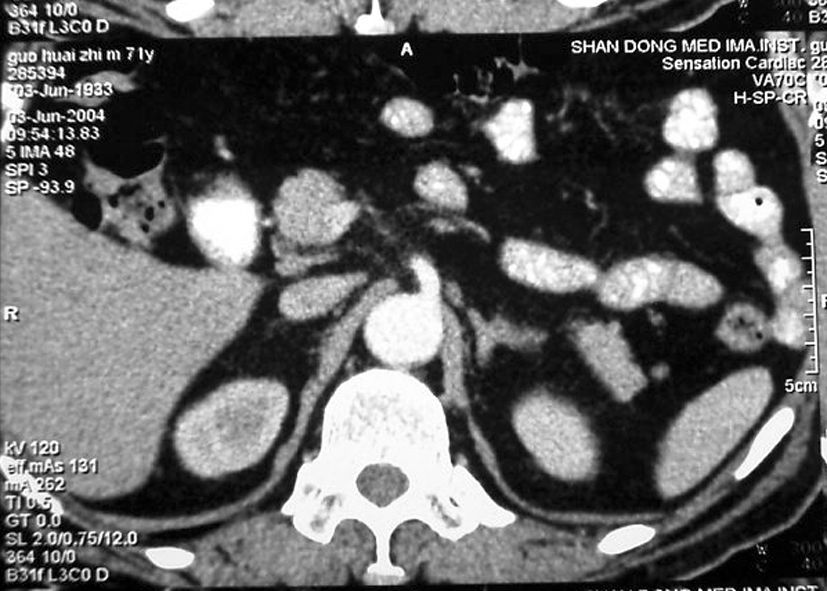
\includegraphics[width=.7\textwidth,height=\textheight,keepaspectratio]{./images/Image00345.jpg}
 \captionsetup{justification=centering}
 \caption{肾上腺增生\\{\small 左侧肾上腺外侧肢呈等密度增粗}}
 \label{fig16-1}
  \end{figure} 

\textbf{【鉴别诊断】}
主要与腺瘤相鉴别。①肾上腺皮质增生症多为双侧病变,可为结节性或弥漫性增生;而肾上腺腺瘤多为单侧发病,且大多是单个病灶。②前者肾上腺外形往往仍保持,只是边缘较丰满而凸出(亦可表现正常);而后者患侧呈肿块状局限突出,且皮质醇腺瘤对侧多萎缩。③前者如呈结节状增生,结节多<1cm,常多发,增强程度与肾上腺一致;而腺瘤多>1cm,且醛固酮腺瘤CT值多≤20Hu,呈轻度强化。④但有时结节状皮质增生与小腺瘤不易鉴别。

此外,有学者指出肾上腺外因素所致的高血压(包括肾性、肾血管性、原发性)患者中,双侧肾上腺可中度增大,这种增大可能是缺血的反应,并不代表其功能亢进。

\subsection{肾上腺皮质腺瘤}

\textbf{【病理】}
多发生于一侧,单发多见。瘤体一般较小。呈圆形或椭圆形,有被膜,生长缓慢,但有恶变的可能性。瘤体内可有出血、坏死液化和囊性变。肿瘤多有分泌功能,并因垂体分泌ACTH受到抑制而使对侧肾上腺萎缩。根据分泌过量的激素不同而分为醛固酮腺瘤、皮质醇腺瘤、肾上腺性征综合征之腺瘤。无功能腺瘤少见,多偶然发现。

\textbf{【临床表现】}
因其分泌的激素不同,临床症状各异(详见概述)。肾上腺瘤以功能性占绝大多数,而无功能性则临床上无肾上腺疾病的症状。

\textbf{【CT表现】}

1.醛固酮腺瘤

有以下特点:肿瘤较小,直径0.8~2.3cm,大多<2cm。呈边缘光滑的圆形或椭圆形。肿瘤密度低(CT值-3~17Hu)是其较特征的CT表现(图\ref{fig16-2})。有报道肾上腺肿瘤平扫CT值≤20Hu时诊断醛固酮腺瘤的敏感性和特异性分别为88%和90%,准确性89%。其CT值较低是因大部分腺瘤细胞浆内充满类脂质颗粒或空泡。肿瘤少有钙化。增强扫描轻度强化或周边环状强化。

\begin{figure}[!htbp]
 \centering
 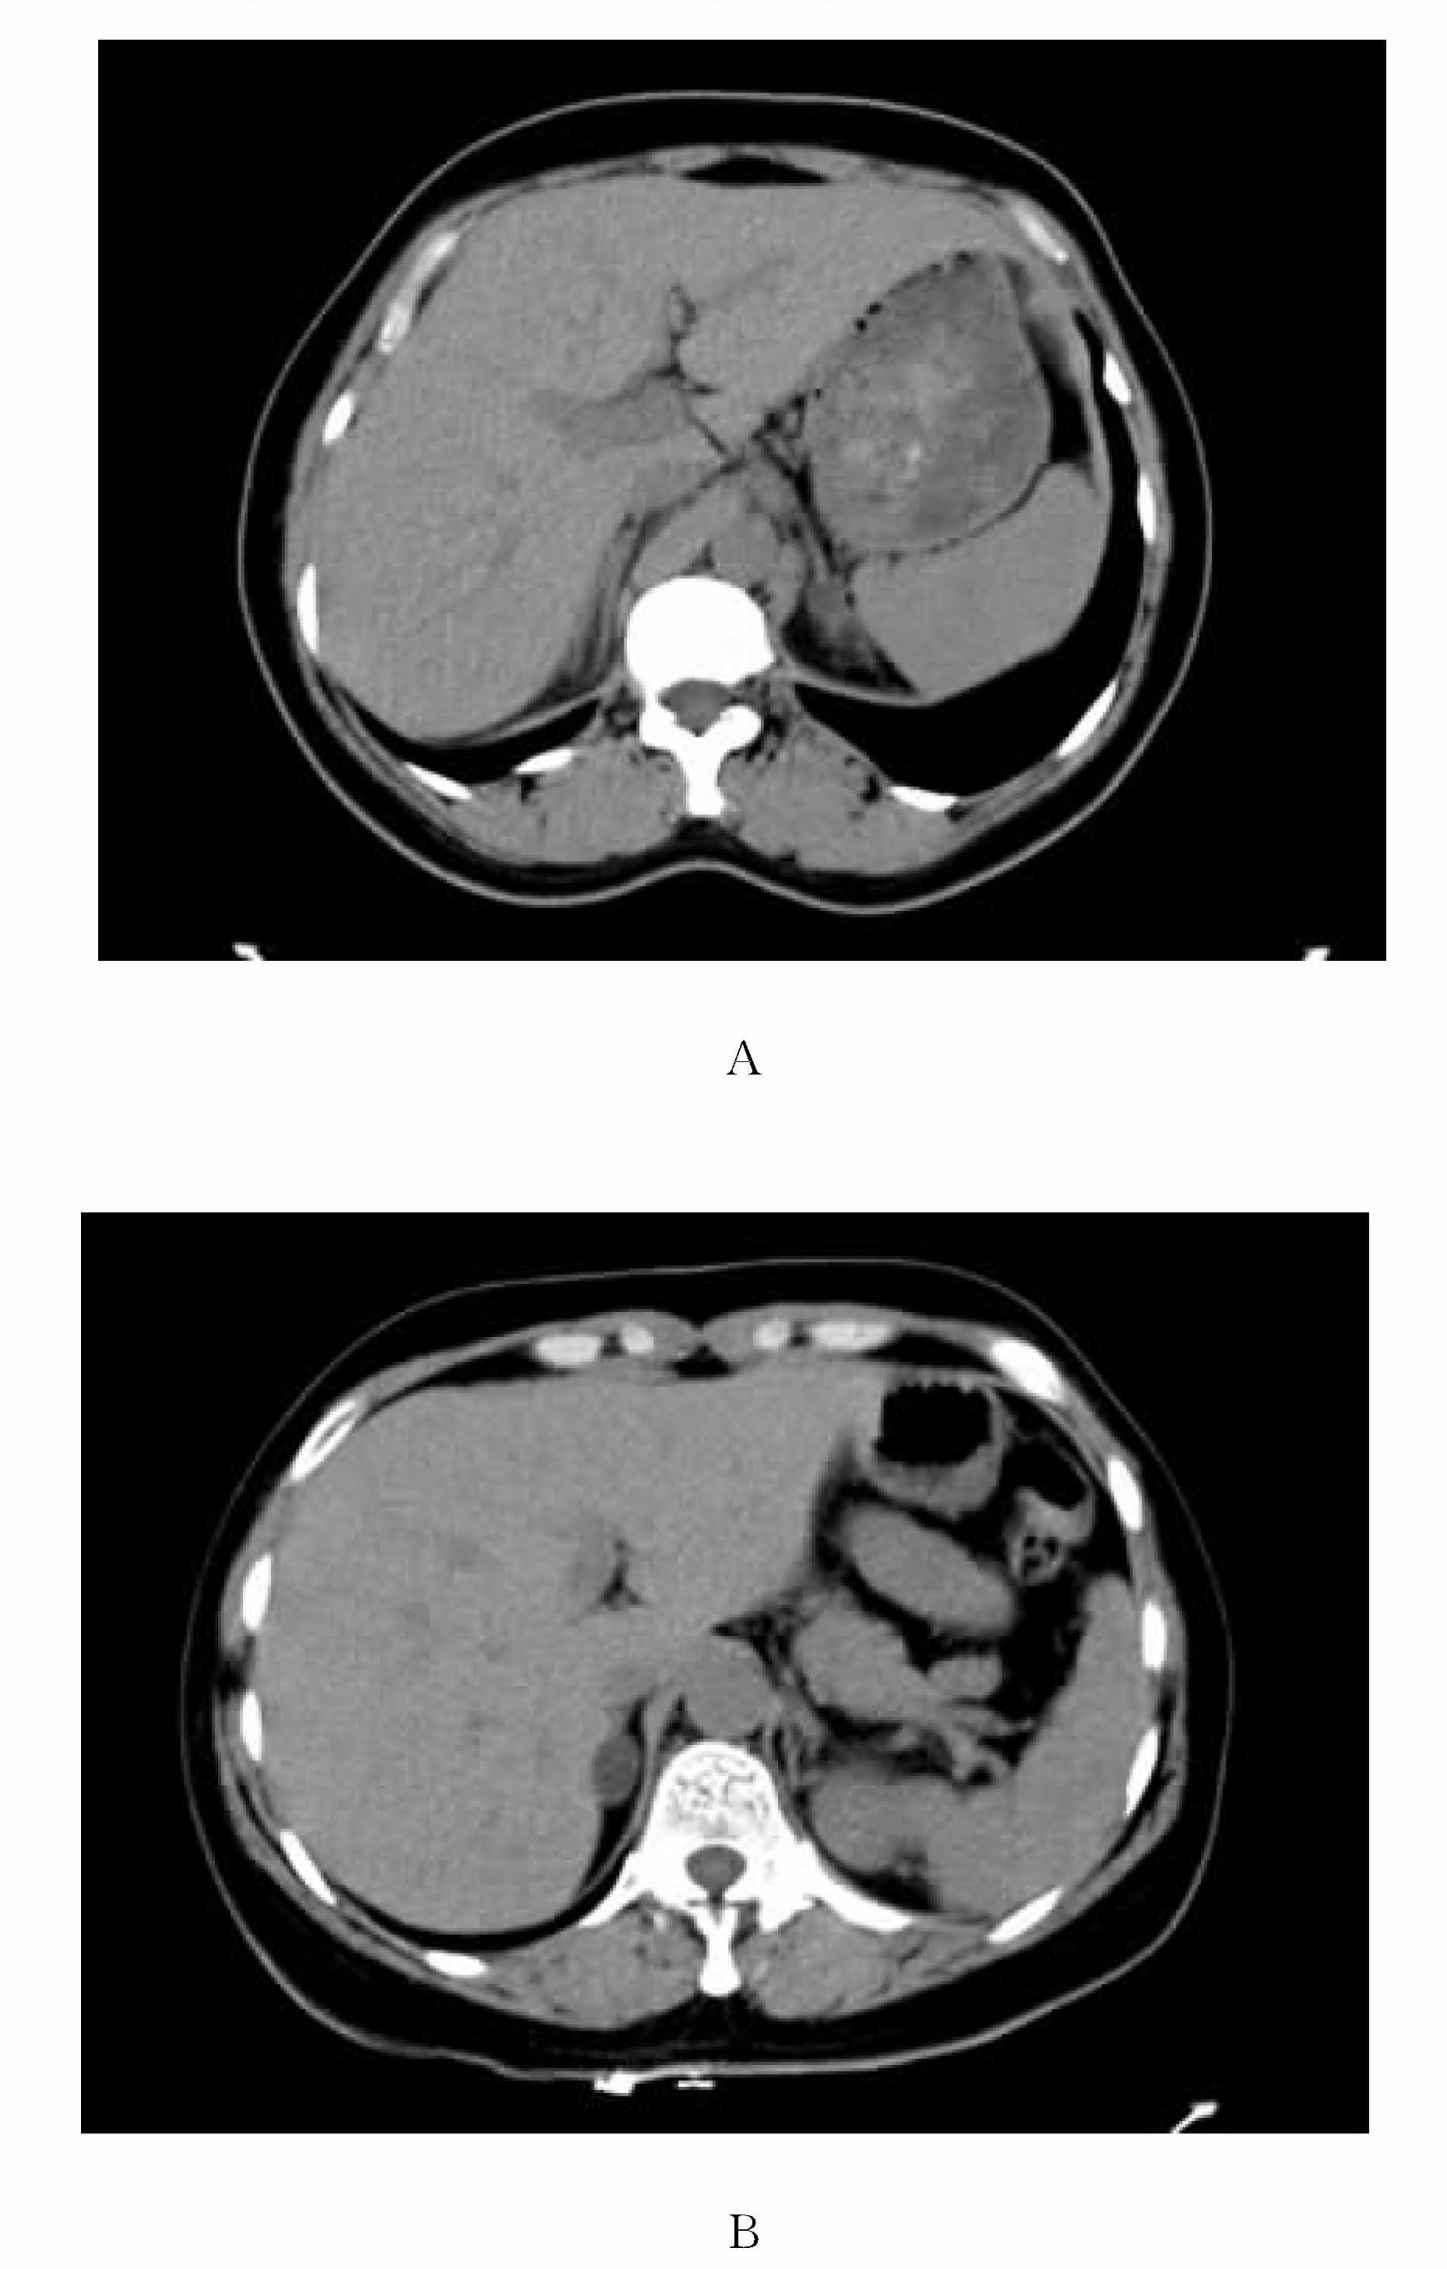
\includegraphics[width=.7\textwidth,height=\textheight,keepaspectratio]{./images/Image00346.jpg}
 \captionsetup{justification=centering}
 \caption{肾上腺皮质腺瘤\\{\small A、B非同一患者,均为醛固酮腺瘤。A肿瘤位于左侧,B肿瘤位于右侧;均呈椭圆形低密度灶,密度均匀,边缘光滑}}
 \label{fig16-2}
  \end{figure} 

2.皮质醇腺瘤

有以下特点:肿块中等大小,直径1.8~4.1cm,大多>2cm。通常呈圆形或椭圆形,边缘清晰。肿瘤密度中等、均匀,很少有钙化。增强扫描可轻度均匀强化,少数不强化。腹膜后脂肪增多,使肿瘤对比明显。另外,对侧肾上腺萎缩亦有助于诊断。

3.肾上腺性征综合征之腺瘤

其CT表现类似皮质醇增多症者。肿瘤呈圆形或椭圆形,边缘清晰,呈恶性发展时可不规则。肿块较大,直径4.3~6.1cm,亦有报道1~10cm不等。分泌雌激素的肿瘤相对更大。肿瘤密度均匀,等密度或略低密度,中心可发生坏死、出血和囊变。增强扫描轻度强化。此外,单侧肾上腺肿瘤病例,其对侧肾上腺可萎缩。

4.无功能性肾上腺腺瘤

肿瘤呈单个圆形,边缘光滑;肿瘤常较大,直径2~10cm。呈略低密度,多密度均匀,CT值取决于其内部含脂肪的多少。少数有钙化。当肿瘤增大明显时可有出血、坏死和囊变。增强扫描轻度强化,对侧肾上腺多正常。与无功能性嗜铬细胞瘤鉴别困难,需依赖病理组织学;与功能性腺瘤的鉴别依靠临床及生化检查。

此外,国内有学者报道,动态增强扫描肾上腺腺瘤表现为廓清迅速,而非腺瘤呈廓清缓慢的特点。

\subsection{肾上腺皮质腺癌}

本病相对少见,功能性和非功能性各占半数。

\textbf{【病理】}
多发生于单侧。瘤体一般巨大。呈圆形、椭圆形或不规则状。瘤体内多有出血、坏死液化、囊性变,少数有钙化。与腺瘤不同的是包膜有浸润、破坏,形态不规则,血管内癌栓形成或远处转移。常较早转移至肝、淋巴结、肺、脑等处。

\textbf{【临床表现】}
常见于男性,多数有腹痛、消瘦、乏力及腹部包块,常因腹部包块就诊。功能性出现相应的临床症状和生化表现,无功能性症状出现较晚。

\textbf{【CT表现】}
肿瘤以左侧多见,10%为双侧受侵。呈不规则或分叶状肿块,边缘模糊。大多数肿瘤体积巨大,直径可达7~20cm。肿瘤常发生出血和坏死而致密度不均匀,少数有钙化。增强扫描强化不明显或呈不均匀强化,亦可呈周边不规则环状强化。常可侵及邻近组织和器官,包括肝、肾及腹膜后淋巴结、肾上腺静脉、肾静脉甚至下腔静脉。

\textbf{【鉴别诊断】}
①腺瘤:显示脏器和淋巴结的转移为恶性的最可靠的依据。但对局限于肾上腺区的占位,区别良恶性有时是困难的。尤其较大的腺瘤亦可有出血、坏死而密度不均,与腺癌不易区分。②转移癌:亦不易鉴别。有学者认为,单发的、直径>5cm,呈不规则强化,有周围结构侵犯或转移时,应考虑皮质腺癌可能;<5cm者难以鉴别。

\subsection{嗜铬细胞瘤}

嗜铬细胞瘤90%发生于肾上腺髓质,其次为肾上腺外的副交感神经节(又称为副神经节瘤),亦可发生于含嗜铬细胞的任何部位。异位的嗜铬细胞瘤常见的部位有肾门、肠系膜根部、腹主动脉旁、膀胱、纵隔等,还有颈部甚至颅内的报道。本病约10%为双侧发病,10%为多发,10%为恶性,10%位于肾上腺外,10%为无功能、无症状性,10%为家族性。本病还可与其他多发神经内分泌瘤相伴发。

\textbf{【病理】}
肿瘤多为球形,呈分叶状并有完整包膜。大小不一,一般体积较大,大多直径>3cm,最大可达20cm。29%伴囊性变,37%伴出血。90%为良性,良、恶性的主要病理区别在于后者血管内癌栓形成、包膜浸润破坏和远处转移,转移处无正常的嗜铬细胞分布。绝大多数嗜铬细胞瘤可被重铬酸钾染色。极少数不被重铬酸钾染色,病理上称为非嗜铬性嗜铬细胞瘤。肿瘤血供丰富。

\textbf{【临床表现】}
本病因瘤细胞分泌肾上腺素和去甲肾上腺素,导致血内儿茶酚胺水平升高,而引起高血压和代谢紊乱为主的临床表现。

1.高血压症候群:①阵发性:占34%;②持续性:占60%。

2.代谢性综合征群:①高血糖和糖尿;②高代谢:脉快、心悸、出汗、震颤、体重减轻和基础代谢升高等,酷似甲状腺功能亢进;③高体温:呈弛张热;④高血钾和高血钙等。

3.全身多系统的影响:主要表现在心血管系统、消化、泌尿、神经代谢方面。

4.实验室检查:尿儿茶酚胺升高,常>17.7μmol/L;尿内儿茶酚胺的代谢产物如甲基肾上腺素和3-甲氧-4-羟苦杏仁酸(VMA)升高,但在发作间隙期可正常。

5.无症状性:部分嗜铬细胞瘤为无功能性或潜在功能性。不发生典型症状的原因除无功能外,亦有人认为其血浆和尿的肾上腺素或去甲肾上腺素虽增多,但其分泌的多巴或多巴胺亦增多,相互作用抵消,故不出现高血压。

\textbf{【CT表现】}
肿瘤呈圆形、椭圆形或梨形、边界清晰的实性肿块,少数为分叶状不规则影。多数边缘光滑。肿瘤较大,直径3~5cm,个别可达20cm。小的肿瘤密度均匀,大者可有坏死、囊变和出血而不均匀;少数肿瘤的中心或边缘可有点状或弧状钙化(图\ref{fig16-3})。增强扫描呈中度到明显强化。除非有邻近组织局部浸润和转移,CT难以鉴别良恶性。但相对来说恶性者瘤体多不规则,坏死、囊变及出血几率更高,与周围组织分界不清。

\begin{figure}[!htbp]
 \centering
 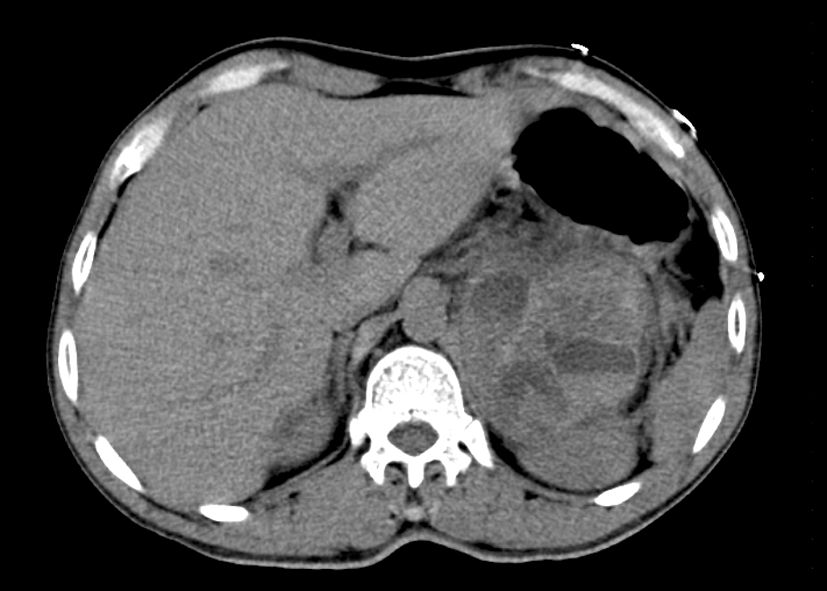
\includegraphics[width=.7\textwidth,height=\textheight,keepaspectratio]{./images/Image00347.jpg}
 \captionsetup{justification=centering}
 \caption{肾上腺嗜铬细胞瘤\\{\small 左肾上腺区有团块状低密度灶,其内有低密度坏死区,病灶界限较清晰}}
 \label{fig16-3}
  \end{figure} 

此外,肾上腺外的异位嗜铬细胞瘤表现为相应部位的软组织肿块,可有明显强化及中心坏死;扫描时应扩大扫描野,依次为肾门区、腹部、盆腔和胸腔。

\subsection{神经母细胞瘤}

本病亦称交感神经母细胞瘤或成神经细胞瘤。本病占儿童肿瘤的10%。主要发生于肾上腺髓质(35%~50%)或腹膜后交感神经节(24%~40%),其次为后纵隔、颈部及内脏交感神经节,甚至可发生于皮下、皮下组织。可为多发性。

\textbf{【病理】}
瘤体多较大,质地较软,常有钙化、坏死和出血。恶性度高,常在短期内突破包膜侵及周围组织器官。镜下典型的为胞质甚少的卵圆形神经母细胞。偶可自发地成熟,由恶性转变为良性的神经节瘤。

转移途径:其恶性程度高,可早期经淋巴及血行转移。常见的转移部位为淋巴结、骨骼和肝脏;肺转移少见,占11%。部分神经母细胞瘤具有分泌功能,可产生肾上腺素、去甲肾上腺素及其前体,以及其他活性物质。

\textbf{【临床表现】}
多发生于婴幼儿,80%发生于5岁以下的幼儿。50%初诊时已有转移。临床以无痛性包块多见。由于转移发生早,表现常多样化,常有消瘦、贫血、淋巴结增大、低热等;因骨转移尤为多见而出现骨痛、运动障碍等,以及脊髓受累症状。75%病人尿中VMA或MHPG升高,尿中多巴胺及HVA增高亦多见,不同于嗜铬细胞瘤。

\textbf{【CT表现】}
肿瘤多呈不规则的实性软组织肿块,常较大。常合并出血、坏死或钙化。钙化以斑点状最为常见,也可为环形或斑块状,化疗后钙化更明显。少数仅为软组织或脂肪密度、无钙化,诊断困难。侵及邻近肾脏时与肾母细胞瘤亦可难以鉴别。此外,还有新生儿囊性神经母细胞瘤的报道,但极为罕见。

\textbf{【鉴别诊断】}

1.肾母细胞瘤:二者均为常见的儿童恶性肿瘤,生长快,瘤体大。肾母细胞瘤少有钙化,与无钙化的神经母细胞瘤区别更为困难。一般认为巨大的神经母细胞瘤虽可压迫肾脏,产生移位,但对肾盂肾盏影响小;而肾母细胞瘤影响肾盂肾盏较多见。有学者认为,腹膜后神经母细胞瘤的分叶征、钙化、腹膜后淋巴结增大和腹主动脉及其分支的包埋等征象有助于与肾母细胞瘤相鉴别。

2.肾上腺神经节瘤:为来源于髓质的良性神经源性肿瘤,多见于女性稍年长儿童。进展缓慢,无转移,几乎无症状,偶然发现。CT表现呈规则的圆形或椭圆形,肿块较大,直径1.6~5.5cm。其密度均匀,由于含脂丰富,肿瘤密度较低,平扫16~41Hu;可有钙化。血供不丰富而强化不著。与神经母细胞瘤的表现有别,但与无功能性腺瘤鉴别困难。

3.神经节母细胞瘤:又称分化性神经母细胞瘤。是既有原始神经母细胞成分,又有节细胞神经瘤成分的恶性肿瘤。常见于10岁以下儿童,偶见于成人。约65%发生于肾上腺外如腹膜后、纵隔和颈部等。确诊需依赖病理组织学。CT示密度不均及周围浸润,伴腹膜后淋巴结肿大,与神经母细胞瘤不易鉴别。

\subsection{肾上腺转移瘤}

本病是肾上腺较为常见的恶性肿瘤之一。

\textbf{【病因病理】}
其原发癌以肺癌和乳癌最为常见,其次为甲状腺癌、胃癌、胰腺癌、结肠癌、恶性黑色素瘤等。有人统计15%~25%的肺癌病例,尤其是小细胞未分化癌,在确诊时已发生肾上腺转移。局部侵犯为转移的另一种方式,相对少见,其中包括肝癌、肾上极癌、恶性淋巴瘤及腹膜后恶性肿瘤。转移癌以双侧发生略多见,其细胞成分与原发癌有关,一般无钙化。

\textbf{【临床表现】}
肾上腺转移癌多为非功能性的,大部分无症状,少数由于双侧腺体破坏严重而继发肾上腺皮质功能减退。

\textbf{【CT表现】}
其表现形式多种多样。转移灶可为单侧或双侧;一般较小,以1~3cm多见,亦可见单侧巨大者(图\ref{fig16-4})。病灶较小时,常呈较均匀的低密度,边缘光滑、清楚,增强扫描呈不同程度的较均匀强化;病灶较大时,密度不均,可有出血、坏死、囊变,边缘不清,增强扫描呈不同程度的不均匀强化,肾上腺结构不清。

\begin{figure}[!htbp]
 \centering
 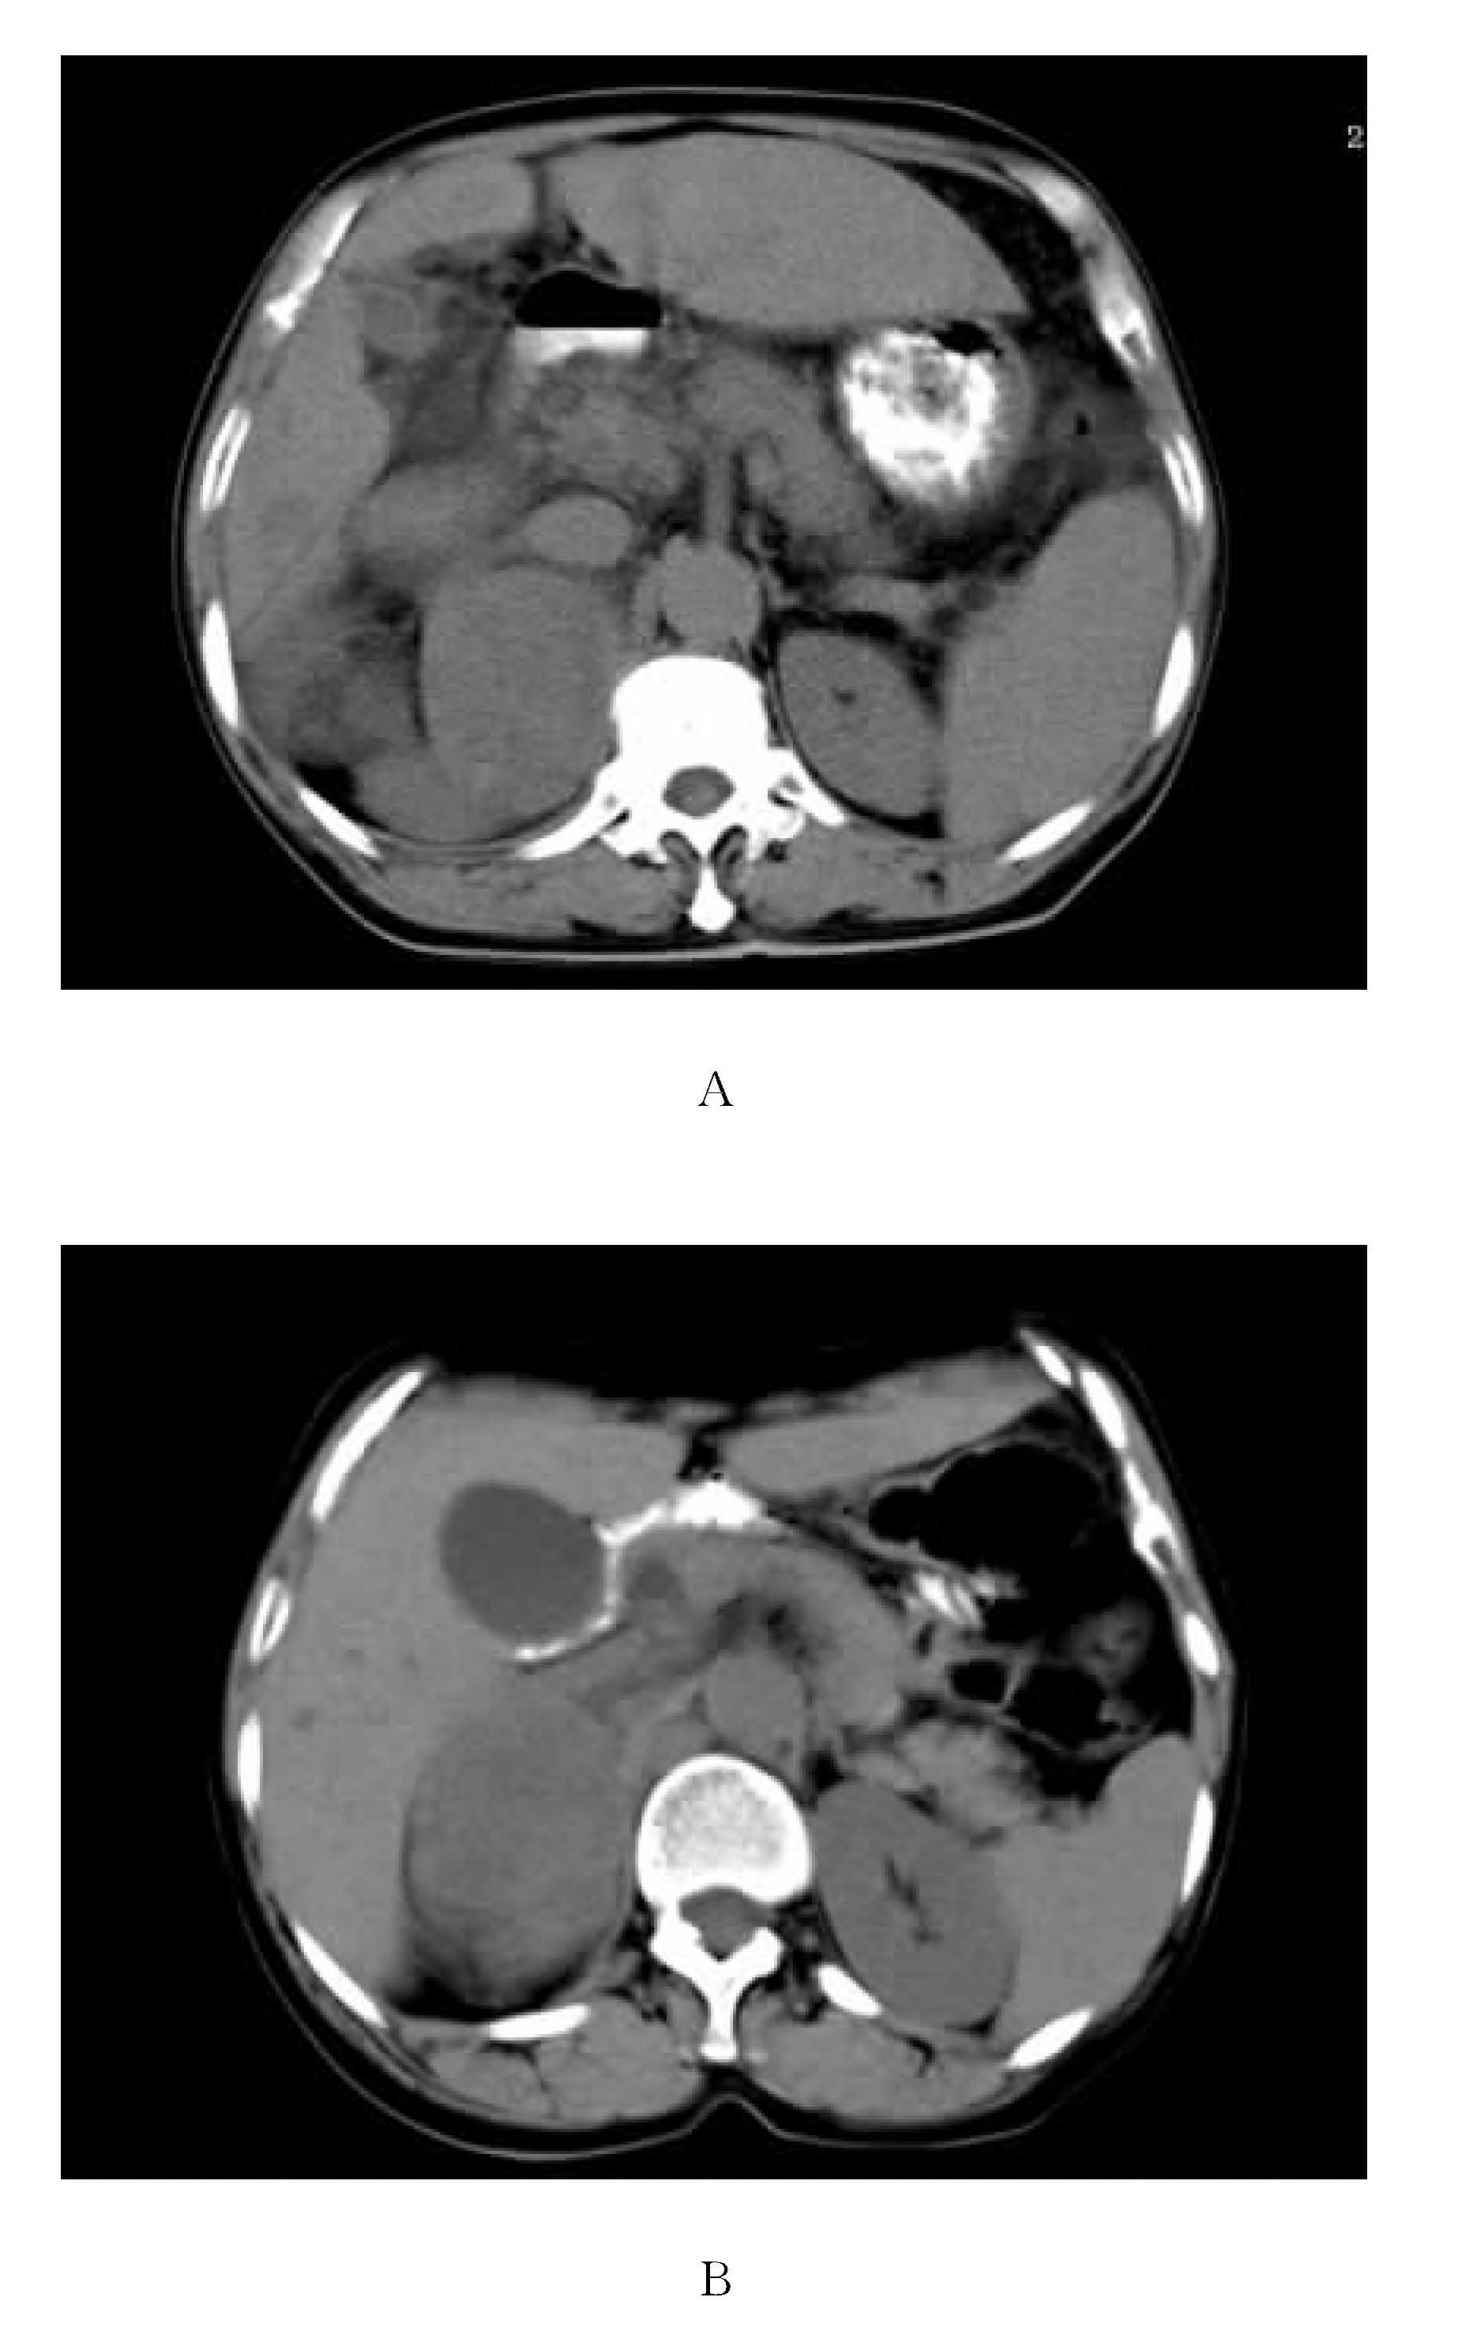
\includegraphics[width=.7\textwidth,height=\textheight,keepaspectratio]{./images/Image00348.jpg}
 \captionsetup{justification=centering}
 \caption{肾上腺转移瘤\\{\small A.肝癌右肾上腺转移;B.肺癌右肾上腺转移}}
 \label{fig16-4}
  \end{figure} 

\textbf{【鉴别诊断】}
与原发性肿瘤(腺瘤或腺癌)的鉴别单靠影像学非常困难,需结合病史。①在已有原发癌的基础上,发现双侧肾上腺占位,应首先考虑为转移瘤;如果肿块为单侧,只能认为转移瘤可能性大,但无法排除肾上腺无功能性腺瘤或腺癌。②当有钙化存在时,应考虑原发性肿瘤可能性大。③在未知原发癌的病例,肾上腺双侧占位多为转移瘤,而单侧占位亦不能排除转移瘤的可能。④个别病例如发现肺孤立性结节和单侧肾上腺占位,如果病理活检为腺癌,有时也难以区分肾上腺病变为原发还是转移。

\subsection{肾上腺髓样脂肪瘤}

本病为少见的无功能性良性肿瘤,发生于皮质或髓质。

\textbf{【病因病理】}
其发病机制可能为毛细血管网状内皮细胞的化生。组织学由比例不一的成熟的骨髓成分和脂肪组织混合组成。肿瘤有残留肾上腺皮质及肾上腺被膜组成的假包膜。镜下见分化良好的脂肪细胞及不同分化的造血干细胞,并有脂肪坏死和出血,偶见钙化,无骨组织。

\textbf{【临床表现】}
本病年龄分布17~93岁,以50~60岁多见,青春期前不发病。多无症状,当肿瘤出血、坏死或因较大压迫邻近脏器时,可出现腹痛、季肋部疼痛等症状。不伴尿常规以及实验室内分泌检查异常。但较大肿瘤压迫肾血管可有高血压,甚至因周围肾上腺组织受刺激增生或萎缩而出现内分泌失调症状。

\textbf{【CT表现】}
肿瘤多为单发,大小不一,一般>3cm。呈圆形,可有分叶,并可见条索状分隔。边界清楚、有包膜。病灶呈密度均匀或不均匀的低密度,多为混杂密度。含脂肪的区域CT值为-30~-100Hu,而其中含骨髓组织的CT值可为13~36Hu。少数可见钙化(20%),呈斑点状或壳状。增强扫描可见肿块内的软组织部分有强化,而脂肪部分几乎无强化(图\ref{fig16-5})。总之,低密度脂肪的存在,是本病的特征性CT表现。

\begin{figure}[!htbp]
 \centering
 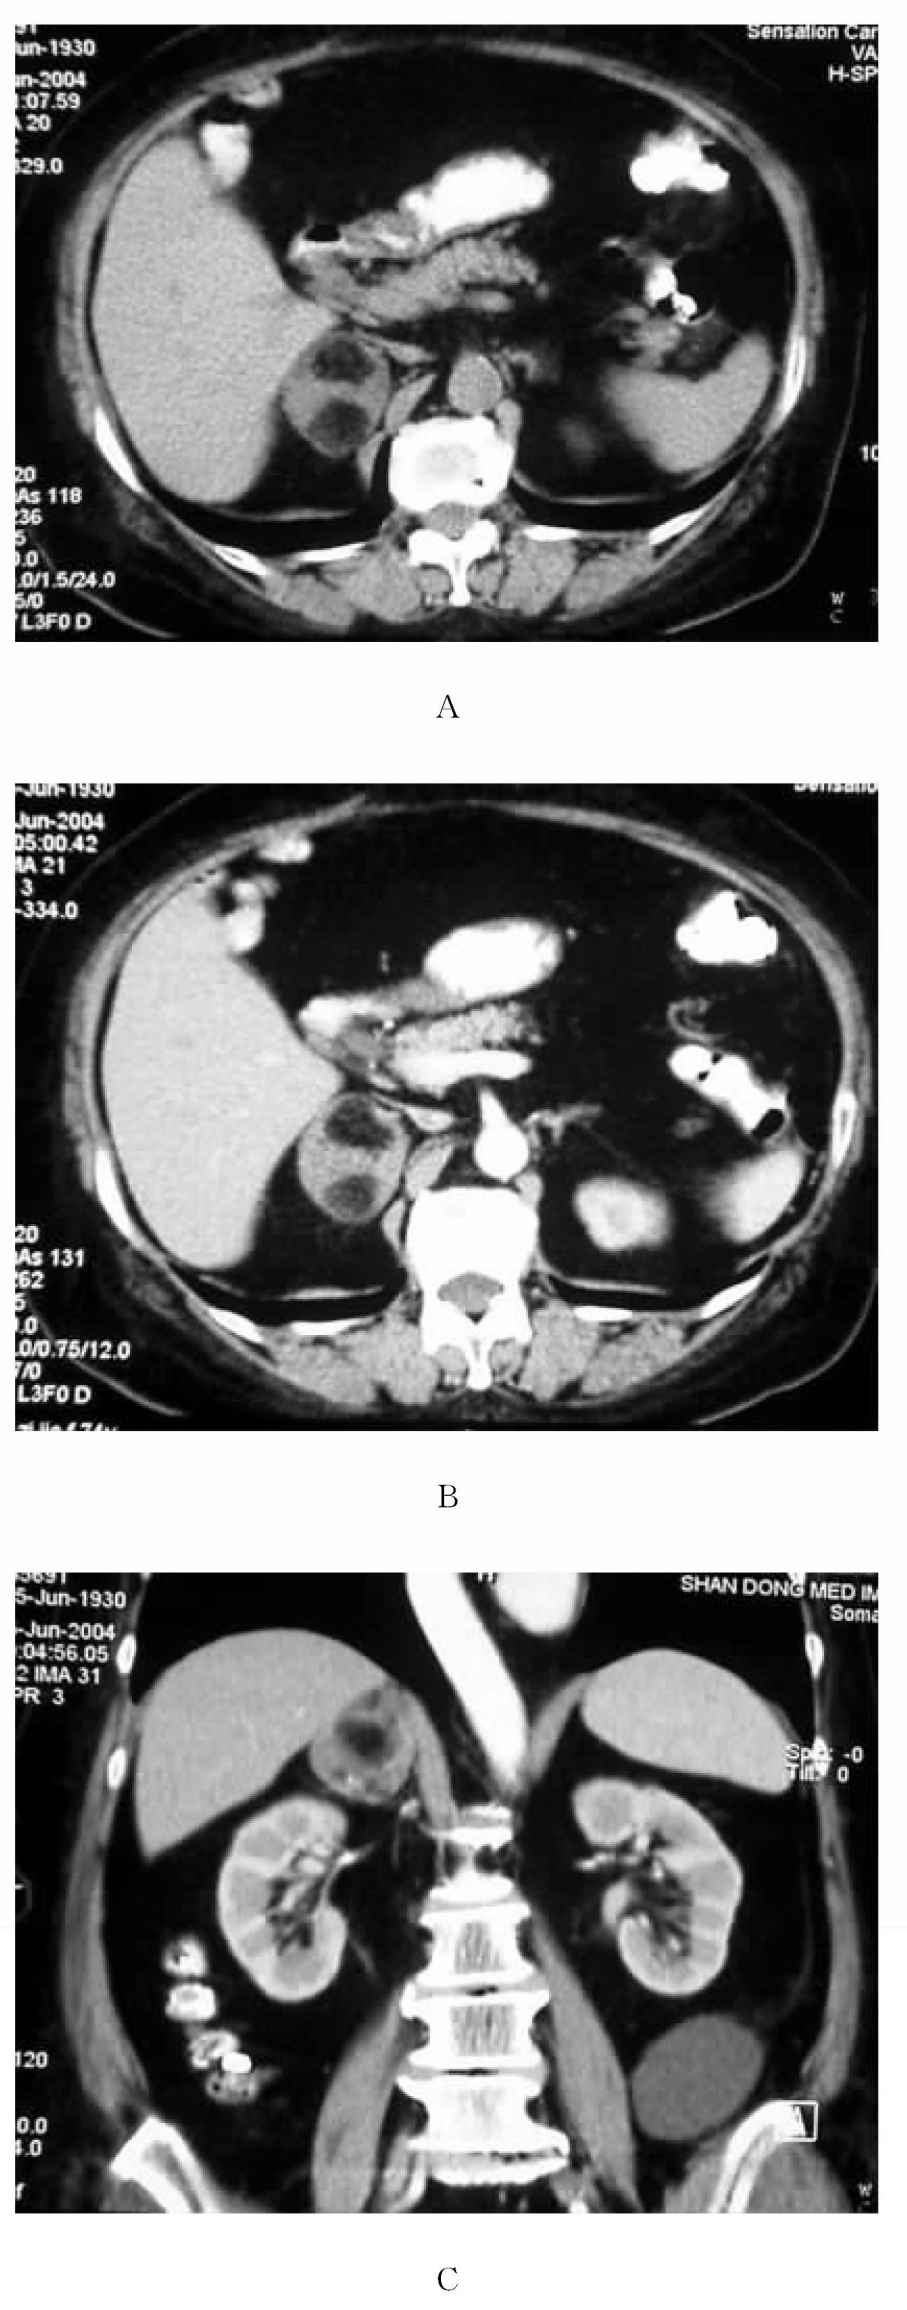
\includegraphics[width=.7\textwidth,height=\textheight,keepaspectratio]{./images/Image00349.jpg}
 \captionsetup{justification=centering}
 \caption{肾上腺髓样脂肪瘤\\{\small A~C为同一患者,A平扫示右侧肾上腺区有椭圆形肿块,其内有两处脂肪低密度区;B、C增强扫描软组织部分有强化,而脂肪部分无明显强化}}
 \label{fig16-5}
  \end{figure} 

\textbf{【鉴别诊断】}
①畸胎瘤:亦为混杂密度,内可见脂肪,但常有斑块状、条片状钙化有助于鉴别。②脂肪瘤:十分罕见,为均匀的脂肪密度,与含有软组织成分的髓样脂肪瘤有别。

\subsection{肾上腺的少见肿瘤}

\subsubsection{起源于肾上腺皮质的间叶性肿瘤}

该类肿瘤甚少见,大多无临床症状。其中,以髓样脂肪瘤略多见(见上述),其次为纤维瘤、脂肪瘤、神经鞘瘤、神经纤维瘤、畸胎瘤、血管瘤、囊肿、淋巴瘤、嗜酸细胞瘤等。

1.血管瘤

罕见,组织学多为海绵状。但常发生纤维性变,有时可为致死性腹膜后出血的原因。

\textbf{【CT表现】}
肿瘤大小不一,可大至6.5cm,偶为双侧。增强扫描肿瘤明显强化。

2.淋巴瘤

极少见,多为NHL,可单侧或双侧肾上腺受累。多见于老年人,临床表现不典型,可有发热、乏力和全身浅表淋巴结增大。

\textbf{【CT表现】}
肿瘤呈单侧或双侧肾上腺巨大软组织肿块,密度均匀或稍不均匀,增强扫描多呈中等均匀或不均匀强化。还可有腹膜后淋巴结增大,肝脏、皮肤受侵,如果伴有脾脏或肾脏弥漫性浸润,则强烈提示淋巴瘤。

3.神经鞘瘤

罕见。为起源于神经外胚层神经鞘细胞的良性肿瘤,可恶变。临床多无症状。

\textbf{【CT表现】}
肿瘤呈较均匀的软组织密度,可伴有囊变,偶见出血、钙化,界限清晰。恶变时,密度多不均匀,有坏死、邻近结构受侵,常伴淋巴结增大。

4.畸胎瘤

极为罕见,多为良性。其发生与胚胎期原始生殖细胞的移行异常有关。由软组织、骨骼、毛发、脂肪等成分构成。

\textbf{【CT表现】}
肿瘤内见软组织、脂肪及骨骼或钙化具有特征性,增强扫描实性部分和分隔略有强化。恶性者可仅有1种组织成分,或以某种成分为主,多为软组织密度肿块,不易鉴别。

5.嗜酸细胞瘤

本病罕见,不合成类固醇激素。属上皮来源,常有完整的纤维包膜。肿瘤质地较均匀,中心常有瘢痕。多无出血、坏死。光镜下肿瘤细胞呈单一的嗜酸细胞,胞浆嗜酸颗粒丰富,偶尔可见核的多形性,核仁明显;电镜下胞浆内充满紧密排列的肿胀线粒体。此病虽为良性,但有潜在恶性行为。

\textbf{【CT表现】}
缺乏特征,与发生于肾的嗜酸细胞瘤相似。表现为界限清楚的实性肿块,多较大,直径常>5cm。病灶中心可有星状瘢痕,多无出血和坏死表现,钙化罕见。

\subsubsection{起源于肾上腺髓质的少见肿瘤}

主要有节细胞神经瘤、神经节母细胞瘤。

1.节细胞神经瘤

是起源于肾上腺髓质及交感神经节的良性肿瘤,由分化好的神经节细胞及神经纤维组成。常发生于纵隔和腹膜后,约20%发生于肾上腺。临床多见于女性,一般无功能,偶然发现。

\textbf{【CT表现】}
平扫肿瘤呈软组织密度,体积较大,其内可见钙化。增强扫描呈进行性轻度延迟强化,动脉期强化轻微而类似囊性肿瘤。

2.神经节母细胞瘤

又称分化性神经母细胞瘤,是既有原始神经母细胞成分,又有节细胞神经瘤成分的恶性肿瘤。约65%发生于肾上腺外如腹膜后、纵隔和颈部等。常见于10岁以下儿童,偶见与成人。预后较神经母细胞瘤好。

\textbf{【CT表现】}
肿瘤密度不均,可有出血、坏死及周围浸润,并可伴腹膜后淋巴结肿大。

\subsection{肝肾间隙巨大占位性病变的定位诊断}

1.肾上腺肿瘤与肝脏肿瘤:①在肿块的中心扫描层面上,肾上腺肿块与肝脏间往往可见脂肪间隙。②下腔静脉移位:肝脏为腹膜腔内脏器,故肝脏肿瘤很少推移下腔静脉,如果出现亦多向后推移;而肾上腺与下腔静脉同位于腹膜后,大的肾上腺肿块多将其向前内推移。③巨大肝癌常侵犯或推移肝内血管,门脉癌栓形成较常见;而肾上腺肿瘤则无此征象。④巨大肾上腺肿瘤可越过中线向对侧生长,而肝右叶肿瘤则一般不跨越中线。

此外,国内有学者报道:肾上腺肿块中心多位于右侧腹中线内侧,且病灶与肝下缘夹角多位于外侧或外侧加内侧;而肝脏肿块多位于右侧腹中线外侧,且病灶与肝下缘夹角多位于内侧。

2.肾上腺肿瘤与肾脏上极肿瘤:①如肿瘤与肾上极的交界面存在,或交角为锐角,则支持来自肾上腺。②肾上腺肿瘤往往将肾脏向下方推移,肾内结构如肾盂肾盏则无改变;相反肾肿瘤往往压迫推移肾盂肾盏,而肾脏本身位置相对无改变。

但个别肾上极肿瘤主要向外生长或肾上腺恶性肿瘤明显侵犯肾脏时,可鉴别困难。

\subsection{肾上腺肿瘤的良恶性鉴别}

肾上腺肿瘤,无论位于皮质和髓质,还是功能和无功能性,均有良恶性之分,但其良恶性的鉴别是有一定困难的。

1.从病理学角度,在细胞形态上不易区分良恶性,诊断恶性肿瘤的标准为包膜和血管受浸润。

2.从CT诊断学及其他影像学角度,显示脏器和淋巴结转移为恶性的最可靠依据。至于肿瘤的大小,及其坏死、出血、囊变和不均匀强化可作为参考征象。一般而言:①轮廓清晰的较小肿瘤,增强前后密度较均匀的,通常为良性。②直径≥5cm的肿瘤,内部密度不均匀,轮廓不清楚的,恶性或潜在恶性的倾向增加。有人认为直径>5cm的无功能性肿瘤以腺癌可能性大。

\section{肾上腺囊肿、血肿及皮质功能减退}

\subsection{肾上腺囊肿}

\textbf{【病因病理】}
可分为4类:①内皮囊肿:约占45%,为发育异常的血管内皮细胞和淋巴管内皮细胞形成的血管样囊肿和淋巴管样囊肿,尤以后者多见。②假性囊肿:约占39%,为各种原因所致的肾上腺出血吸收后的结果,这种出血可发生于正常肾上腺出血或肾上腺肿瘤出血。③上皮囊肿:约占9%,囊肿内壁为柱状上皮,包括真性腺样囊肿、胚胎性囊肿和囊性肾上腺肿瘤。④寄生虫囊肿:约占7%,主要源于细粒棘球绦虫感染即包虫病。

\textbf{【临床表现】}
本病绝大多数无临床症状,较大者可出现周围组织器官受压改变、腹痛及腹块。

\textbf{【CT表现】}
囊肿多呈圆形或椭圆形,边缘清楚,密度均匀,一般体积较小(图\ref{fig16-6})。CT值取决于囊内容物蛋白质含量,通常为0~20Hu,囊内合并出血时,CT值可升高。囊肿可为单房、双房或多房,囊壁薄而均匀,厚度不超过2~3mm。肿瘤源性囊肿,壁厚薄不均。约15%囊壁有弧形和斑点状钙化,尤其是出血后囊肿。增强扫描囊肿无强化。

\begin{figure}[!htbp]
 \centering
 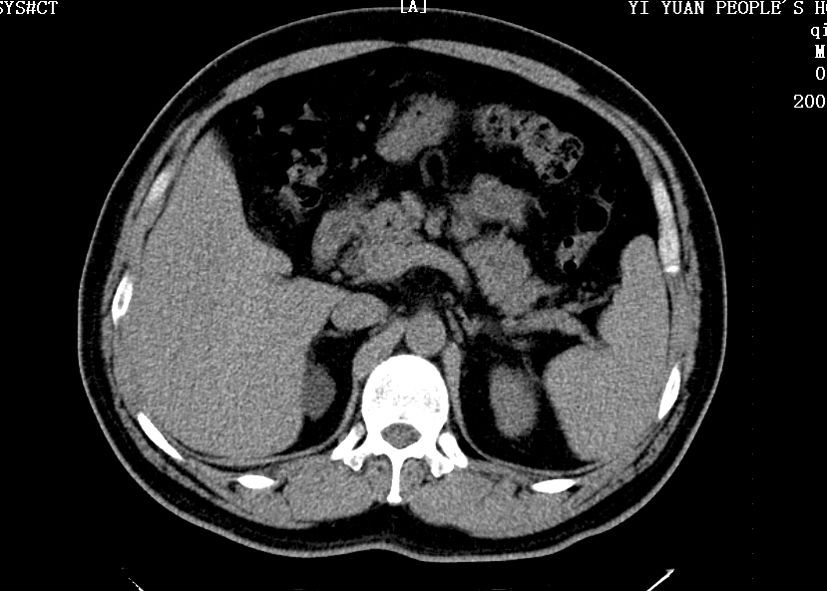
\includegraphics[width=.7\textwidth,height=\textheight,keepaspectratio]{./images/Image00350.jpg}
 \captionsetup{justification=centering}
 \caption{右侧肾上腺囊肿\\{\small 右肾上腺区椭圆形水样密度灶,边缘光滑锐利(B超证实为液性无回声灶)}}
 \label{fig16-6}
  \end{figure} 

\subsection{肾上腺出血和血肿}

本病少见,多见于外伤及其他的应急状态。

\textbf{【病因病理】}
引发出血的原因为败血症、休克、创伤、出血体质、抗凝血治疗、肿瘤、手术以及严重的应激反应。新生儿肾上腺出血与围产期窒息缺氧、酸中毒、应激、产伤和继发循环障碍密切相关,多为单侧性、局限性。双侧弥漫性多与抗凝治疗不当有关。肾上腺可发生自发性出血,有人认为右侧较左侧多见,可能由于右肾上腺静脉直接注入下腔静脉,血压升高可直接传导至右肾上腺静脉所致。肾上腺出血可为急性、亚急性和慢性;约20%以上为双侧性。

\textbf{【临床表现】}
可有腹部、背部、肋部及下胸部疼痛,甚至出现剧烈腹痛,腹肌紧张、压痛和反跳痛,同时伴恶心、呕吐等为胃肠道症状。严重者可有肾上腺危象的表现,如低血压、休克和心动过速及发热等。新生儿可出现腹块、黄疸、休克等症状和体征。

\textbf{【CT表现】}
平扫可见肾上腺肿胀,密度增高,呈条状阴影延伸到肾上腺周围结构内(图\ref{fig16-7})。当出血较大时可积聚形成血肿,血肿多见于肾上腺髓质。出血和血肿急性期为高密度,随着时间推移,肾上腺体积缩小、密度减低。出血和血肿的吸收大约在6周以后,3~6个月后可完全吸收;少数不完全吸收或机化时,可见条状软组织影或钙化。

\begin{figure}[!htbp]
 \centering
 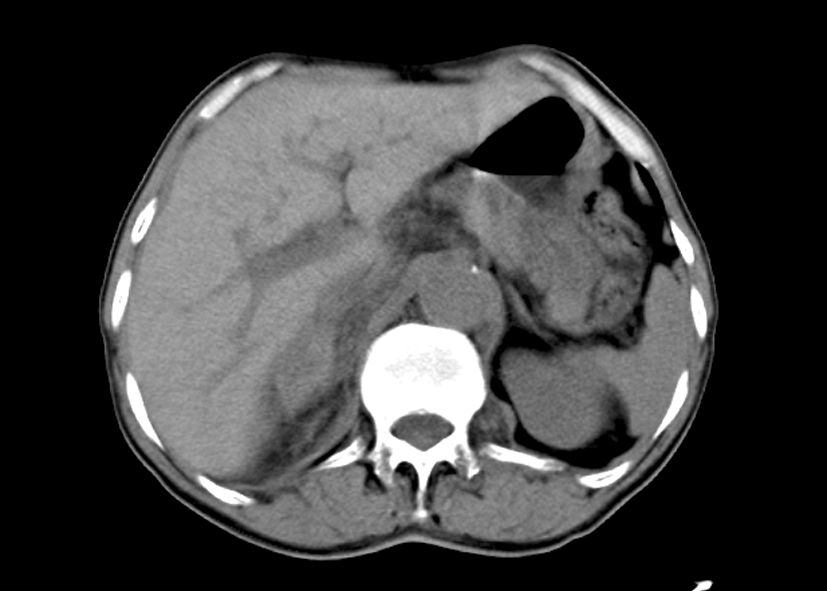
\includegraphics[width=.7\textwidth,height=\textheight,keepaspectratio]{./images/Image00351.jpg}
 \captionsetup{justification=centering}
 \caption{右侧肾上腺血肿\\{\small 外伤患者,右侧肾上腺区有椭圆形稍高密度灶,界限欠清晰;局部还有许多条索状高密度灶}}
 \label{fig16-7}
  \end{figure} 

\subsection{肾上腺结核}

原发性很少见,多继发于其他脏器结核,由血行播散所致。

\textbf{【病理】}
多是双侧病变,可单侧发病。可分为干酪化期和钙化期。早期结核菌侵及肾上腺,破坏皮质和髓质,形成结核性肉芽肿或以干酪坏死为主,其后淋巴细胞和巨细胞浸润,最终发生钙化。常与肾结核、腹膜结核和附睾结核同时存在。

\textbf{【临床表现】}
起病缓慢。主要表现为肾上腺皮质功能减退症状,如乏力、恶心、呕吐、体重下降、皮肤色素沉着(尤以暴露部位为著)等。随病情进展,上述症状加重。尿中17-羟皮质类固醇减低,结核中毒症状多不明显。

\textbf{【CT表现】}
国内有学者分为3期。Ⅰ期:双侧肾上腺增大,形成卵圆形或三角形肿块,但仍具有正常肾上腺分支结构。钙化出现率低,且较细微。可有局限性低密度,增强扫描常呈单环状或多环状强化,无强化区代表干酪样坏死灶。少数无明确低密度区,呈轻度强化,代表以结核性肉芽肿为主。此期病程多在1年之内。Ⅱ期:双侧肾上腺明显增大,形态相对不规则,无局限性低密度。钙化常见且较粗糙,呈散在分布。此期病程在1~4年之间。Ⅲ期:肾上腺大小正常或萎缩,失去正常肾上腺形态,钙化呈致密斑片状。此时病程多在4年以上。

国内还有学者报道,进展期病灶多表现为密度不均,增强扫描明显环状强化;稳定期病灶纤维化、钙化明显,且不强化。有利于指导临床治疗。

\subsection{肾上腺皮质功能减退症}

1.根据病因分为:①原发性:主要为自身免疫性疾病,以自身免疫性肾上腺炎、多腺体自身免疫综合征最为常见;其次为感染性因素,以结核多见,也可由于真菌、梅毒、艾滋病引起;此外肾上腺原发性或继发性肿瘤、淀粉样变性、肾上腺严重出血坏死后、手术等。②继发性:主要为垂体肿瘤、坏死、先天缺陷等垂体病变所致的ACTH分泌减少等;其次为长期应用肾上腺皮质激素所致。

2.根据病程分为:①急性:大都由于严重感染、外伤、手术或长期激素治疗造成下丘脑-垂体分泌ACTH功能抑制,ACTH分泌减少,引起继发性肾上腺皮质萎缩。在严重感染时,肾上腺皮质和髓质见大片状出血,导致急性皮质功能不足。②慢性:慢性肾上腺皮质功能减退亦称为Addison's病。是由于肾上腺结核或自然免疫等原因破坏了双侧肾上腺皮质,激素分泌不足所致。

\textbf{【临床表现】}
主要表现为血压降低、虚弱无力、恶心、呕吐、低血糖、抵抗力降低和皮肤色素沉着等。严重者出现休克及神经系统症状。

\textbf{【CT表现】} 结核性见上述,其部分少见病变的CT表现如下:

1.自身免疫性:可伴有其他自身免疫性疾病。CT表现为肾上腺70%萎缩(多为幼儿患者或幼时起病的成年患者),30%正常或增大。无钙化及低密度区。

2.真菌性:肾上腺增大,多无钙化,早期抗真菌治疗有效。但组织胞浆菌病可见双侧肾上腺增大,内有低密度区和钙化,与结核难以鉴别。

3.肿瘤性:双侧肾上腺转移瘤或淋巴瘤,表现双侧肾上腺不规则增大等。

4.淀粉样变性:罕见,可有肾上腺的增大、钙化。其确诊需穿刺活检。

\protect\hypertarget{text00024.html}{}{}

